%%%%%%%%%%%%%%%%%%%%%%%%%%%%%%%%%%%%%%%%% 
% Beamer Presentation
% LaTeX Template
% Version 1.0 (10/11/12)
% 
% This template has been downloaded from:
% http://www.LaTeXTemplates.com
% 
% License:
% CC BY-NC-SA 3.0 (http://creativecommons.org/licenses/by-nc-sa/3.0/)
% 
%%%%%%%%%%%%%%%%%%%%%%%%%%%%%%%%%%%%%%%%% 

% ----------------------------------------------------------------------------------------
%	PACKAGES AND THEMES
% ----------------------------------------------------------------------------------------

\documentclass{beamer}

\mode<presentation> {

  % The Beamer class comes with a number of default slide themes
  % which change the colors and layouts of slides. Below this is a list
  % of all the themes, uncomment each in turn to see what they look like.

  % \usetheme{default}
  % \usetheme{AnnArbor}
  % \usetheme{Antibes}
  % \usetheme{Bergen}
  % \usetheme{Berkeley}
  % \usetheme{Berlin}
  % \usetheme{Boadilla}
  % \usetheme{CambridgeUS}
  % \usetheme{Copenhagen}
  % \usetheme{Darmstadt}
  % \usetheme{Dresden}
  % \usetheme{Frankfurt}
   \usetheme{Goettingen}
  % \usetheme{Hannover}
  % \usetheme{Ilmenau}
  % \usetheme{JuanLesPins}
  % \usetheme{Luebeck}
  % \usetheme{Madrid}
  % \usetheme{Malmoe}
  % \usetheme{Marburg}
  % \usetheme{Montpellier}
  % \usetheme{PaloAlto}
  % \usetheme{Pittsburgh}
  % \usetheme{Rochester}
  % \usetheme{Singapore}
  % \usetheme{Szeged}
  % \usetheme{Warsaw}

  % As well as themes, the Beamer class has a number of color themes
  % for any slide theme. Uncomment each of these in turn to see how it
  % changes the colors of your current slide theme.

  % \usecolortheme{albatross}
  % \usecolortheme{beaver}
  % \usecolortheme{beetle}
  % \usecolortheme{crane}
  % \usecolortheme{dolphin}
  % \usecolortheme{dove}
  % \usecolortheme{fly}
  % \usecolortheme{lily}
  % \usecolortheme{orchid}
  % \usecolortheme{rose}
  % \usecolortheme{seagull}
  % \usecolortheme{seahorse}
  % \usecolortheme{whale}
  % \usecolortheme{wolverine}

  % \setbeamertemplate{footline} % To remove the footer line in all slides uncomment this line
   \setbeamertemplate{footline}[page number] % To replace the footer line in all slides with a simple slide count uncomment this line

  % \setbeamertemplate{navigation symbols}{} % To remove the navigation symbols from the bottom of all slides uncomment this line
}

\usepackage{graphicx} % Allows including images
\usepackage{booktabs} % Allows the use of \toprule, \midrule and \bottomrule in tables
\usepackage[german]{babel} % Required to compile in Windows
\usepackage[latin1]{inputenc}
\usepackage{caption}
\usepackage{subcaption}
%\usepackage{physics}
\usepackage{mathtools}
\usepackage{natbib}
\usepackage[T1]{fontenc}


\AtBeginSection[]{
  \begin{frame}
    \vfill
    \centering
    \begin{beamercolorbox}[sep = 8pt, center, shadow = true, rounded = true]{title}
      \usebeamerfont{title}\insertsectionhead\par%
    \end{beamercolorbox}
    \vfill
  \end{frame}
}

% ----------------------------------------------------------------------------------------
%	TITLE PAGE
% ----------------------------------------------------------------------------------------

\title[]{Projekt 1a: Die Projektvorstellung} % The short title appears at the bottom of every slide, the full title is only on the title page

\author{Isabell Albrecht, Erik Engelhardt, Oliver Kochan, Florian Steffens} % Your name
\institute[HAW] % Your institution as it will appear on the bottom of every slide, may be shorthand to save space
{
  Hochschule f�r angewandte Wissenschaften -- Hamburg \\ % Your institution for the title page
  \medskip
  %\textit{erik.engelhardt@haw-hamburg.de, hier@email.eintragen} % Your email address
}

\date{\today} % Date, can be changed to a custom date

\begin{document}

\begin{frame}
  \titlepage % Print the title page as the first slide
\end{frame}

\section{Einleitung}
% - Gruppenmitglieder vorstellen
% - welches Projekt bearbeiten wir (Bild)
\begin{frame}
  \frametitle{Wetterstation - Projekt 1a}
  \begin{figure}
    \centering
    \begin{minipage}[t]{0.45\linewidth}
        \centering
        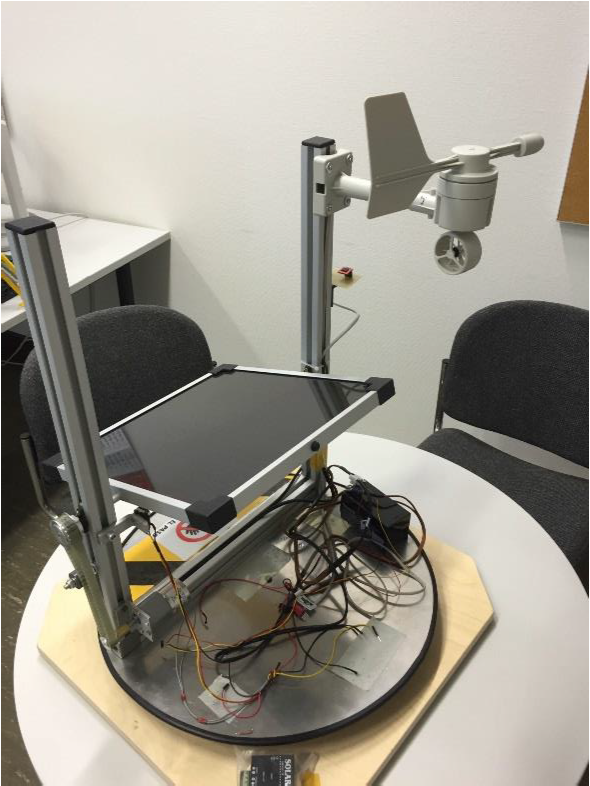
\includegraphics[width=\linewidth]{img/Wetterstation_1.png}
    \end{minipage}% <- sonst wird hier ein Leerzeichen eingef�gt
    \hfill
    \begin{minipage}[t]{0.45\linewidth}
        \centering
        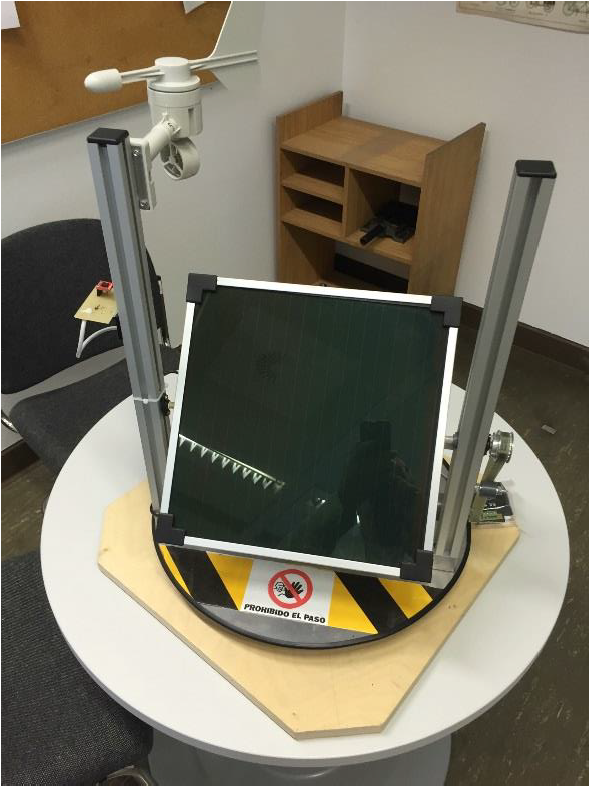
\includegraphics[width=\linewidth]{img/Wetterstation_2.png}
    \end{minipage}
    \end{figure}
  %\emph{Diese Wetterstation wird sehr gut.}
\end{frame}

\begin{frame}[allowframebreaks]
  %\frametitle{Gliederung} % Table of contents slide, comment this block out to remove it
  \tableofcontents % Throughout your presentation, if you choose to use \section{} and \subsection{} commands, these will automatically be printed on this slide as an overview of your presentation
\end{frame}

% ----------------------------------------------------------------------------------------
%	PRESENTATION SLIDES
% ----------------------------------------------------------------------------------------

\section{Anforderungen}
% - zusammenfassen der Puntke aus Vorlage
% - eingrenzung Messbereiche
\subsection{Anforderungen aus Pflichtenheft}
\begin{frame}
  \frametitle{Anforderungen aus Pflichtenheft 1/2}
  \emph{Datenerfassung}
  \begin{itemize}
  	\item \emph{Temperatur �ber mind. 2 Sensoren}
  	\item \emph{Luftdruck}
  	\item \emph{Luftfeuchtigkeit}
  	\item \emph{H�he �ber NN}
  	\item \emph{Windrichtung}\\
  \end{itemize}
\end{frame}
\begin{frame}
  \frametitle{Anforderungen aus Pflichtenheft 2/2}
  \emph{Weitere Anforderungen}
  \begin{itemize}
  
  	\item \emph{Versorgung �ber Solarenergie}
  	\item \emph{Akkupufferung}
  	\item \emph{Erfassung des Akku-Zustands (Spannung und Strom)}
  	\item \emph{Nachgef�hrte Solarenergie}
  	\item \emph{Automatische Ausrichtung des Solarpanels}
  	\item \emph{Positionsbestimmung}
  	\item \emph{Datenspeicherung auf einer microSD-Karte}
  	\item \emph{Drahtlose Kommunikation mit einem PC}
  	
  	
  \end{itemize}
\end{frame}
\subsection{Abgeleitete Anforderungen}
\begin{frame}
  \frametitle{Abgeleitete Anforderungen}
  \emph{Zus�tzlich ergibt sich:}
  \begin{itemize}
  	\item \emph{Temperaturerfassung von -60 bis 60\ �C}
  	\item \emph{Luftfeuchtigkeit von 0 bis 100\ \%}
  	\item \emph{Luftdruck von 325,4 (Totes Meer) bis 1070\ hPa (Mount Everest)}
  	\item \emph{Wasserdichter Aufbau}
  	\item \emph{Energiesparender Messaufbau (Sleep Mode)}
  \end{itemize}
\end{frame}
%\section{Konzept} %keine Ahnung, was ich hier schreiben soll :)
% - Blockschaltbild
%\begin{frame}
  %\frametitle{Folie 1}
  %\emph{Diese Wetterstation wird sehr gut.}
 
%\end{frame}
\section{Umsetzung}
% - Sensoren kurz vorstellen und Bezug auf Anforderungen nehmen
\begin{frame}
  \frametitle{Sensoren}
  \subsection{Sensoren}
        \emph{Bosch Sensortec }\href{https://www.bosch-sensortec.com/bst/products/all_products/bme280}{\textbf{BME280}}
        \begin{itemize}
            \item \emph{Luftdruck-, Luftfeuchte- und Temperatursensor}
           	\item \emph{Luftdruck von 300 bis 1100\ hPa}
           	\item \emph{Temperatur von -40 bis 60\ �C}
           	\item \emph{Luftfeuchtigkeit von 0 bis 100\ \%}
           	\item \emph{Arbeitsbereich von -40 bis 85\ �C}
         \end{itemize}
         \begin{figure}
         	\flushright         
         	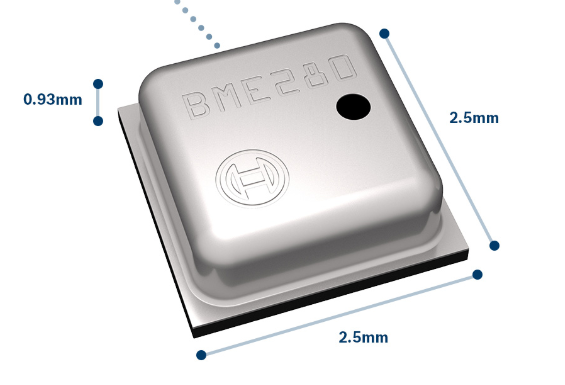
\includegraphics[width=0.5\linewidth]{img/BME280.png}
         \end{figure}
\end{frame}

\begin{frame}
	\frametitle{Sensoren}
	\emph{Honeywell} \href{https://www.sparkfun.com/datasheets/Components/HMC6352.pdf}{\textbf{HMC6352}}
	\begin{itemize}
		\item \emph{Magnetometer mit DSP-ASIC}
		\item \emph{Arbeitsbereich von -20 bis 70\ �C}
		\item \emph{Ausrichtung der Wetterstation}
		\end{itemize}
	\begin{figure}
         	\flushright         
         	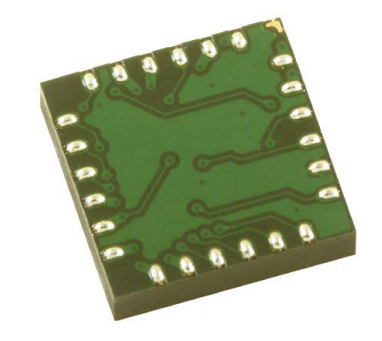
\includegraphics[width=0.5\linewidth]{img/HMC6352.png}
    \end{figure}
\end{frame}
 
\begin{frame}
	\frametitle{Sensoren}
	\emph{ST Microelectronics} \href{https://www.st.com/en/mems-and-sensors/lis3dh.html}{\textbf{LIS3DH}}
	\begin{itemize}
		\item  \emph{MEMS-Accelerometer und Temperatursensor}
		\item  \emph{Mess- und Arbeitsbereich von -40 bis 85\ �C}
		\item \emph{Ausrichtung des Solarpanels}
	\end{itemize}

	\emph{Allegro} \href{https://www.allegromicro.com/en/products/sense/current-sensor-ics/zero-to-fifty-amp-integrated-conductor-sensor-ics/acs712}{\textbf{ACS712}}
	\begin{itemize}
		\item \emph{Halleffekt-Stromsensor}
		\item \emph{Bestimmung des Ladezustands des Bleiakkus}
	\end{itemize}
	\begin{figure}
         	\flushright         
         	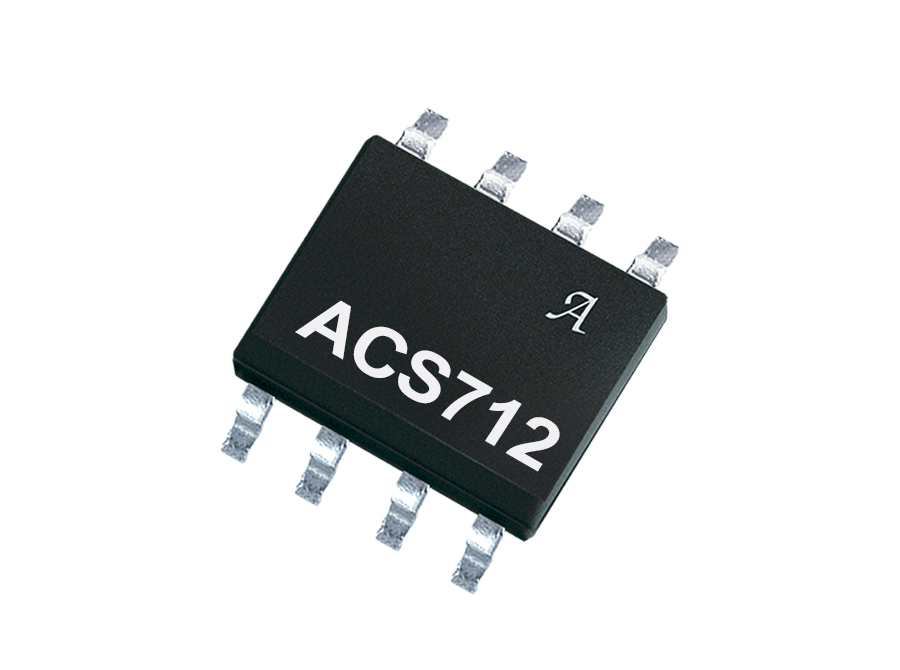
\includegraphics[width=0.5\linewidth]{img/ACS712.jpg}
    \end{figure}
\end{frame}

\begin{frame}
	\frametitle{Sensoren}
    \emph{Sparkfun} \href{https://www.sparkfun.com/products/8942}{\textbf{SEN-08942}}
    \begin{itemize}           
            \item \emph{Anemometer, Windfahne und Niederschlagssensor}
            \item \emph{einfachere Implementierung als vorgegebener Sensor}
    \end{itemize}
    \begin{figure}
         	\flushright         
         	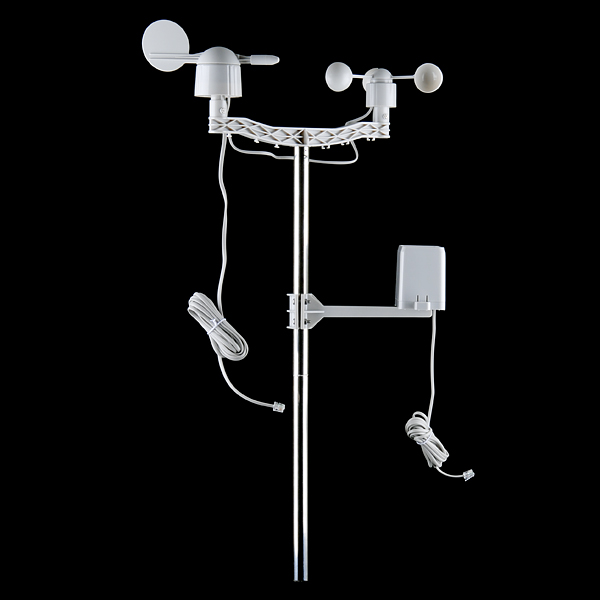
\includegraphics[width=0.5\linewidth]{img/SEN-08942.jpg}
    \end{figure}
\end{frame}

\begin{frame}
    \frametitle{Kommunikation und Leistungselektronik}
    \subsection{Kommunikation, LE}
        \emph{SkyTraq \href{}{\textbf{Venus600 series}}}
        \begin{itemize}
        	\item \emph{GPS Empf�nger-ASIC}
        	\item \emph{Standort- und Uhrzeitbestimmung}
        	\item \emph{Zusammen mit Accelerometer und Kompassmodul Ausrichtung des Solarpanels}
        \end{itemize}
        \emph{``no-name'' \textbf{HC-05}}
        \begin{itemize}
            \item \emph{Serial-over-Bluetooth Schnittstellenumsetzer}
            \item \emph{Kommikation mit Display (optional)}
        \end{itemize}
        \emph{ST Microelectronics \href{https://www.st.com/en/motor-drivers/l293e.html}{\textbf{L293E}}: Motortreiber} \\
        \emph{IVT \textbf{200007}: MPPT Laderegler}
\end{frame}

\begin{frame}
\frametitle{Energieversorgung}
    \subsection{Versorgung}
        Autarke Energieversorgung:
        \begin{itemize}
            \item \emph{Sygonix \textbf{SY-VRU214-4}: Solarmodul}
            \item\emph{``no-name'' Blei-S�ure Sekund�rzelle}
        \end{itemize}
        \begin{figure}
    \centering
    \begin{minipage}[t]{0.45\linewidth}
        \centering
        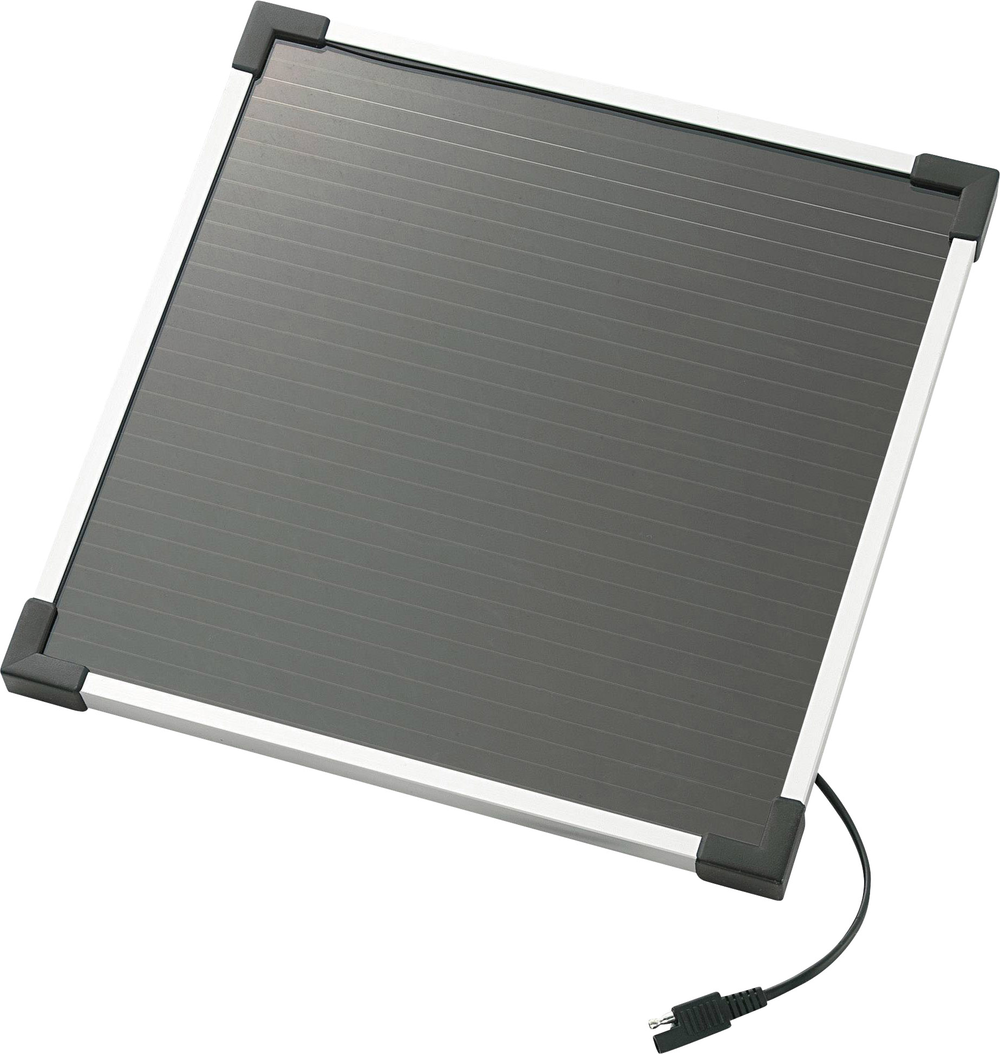
\includegraphics[width=\linewidth]{img/SY-VRU214-4.png}
    \end{minipage}% <- sonst wird hier ein Leerzeichen eingef�gt
    \hfill
    \begin{minipage}[t]{0.45\linewidth}
        \centering
        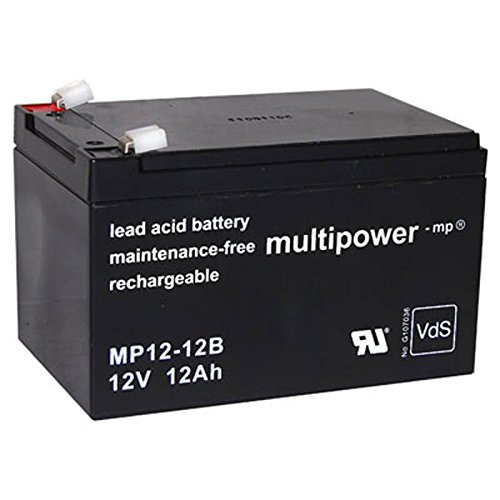
\includegraphics[width=\linewidth]{img/Bleiakku.jpg}
    \end{minipage}
    \end{figure}
\end{frame}
\begin{frame}
\frametitle{System�bersicht}
    \subsection{Aufbau}
        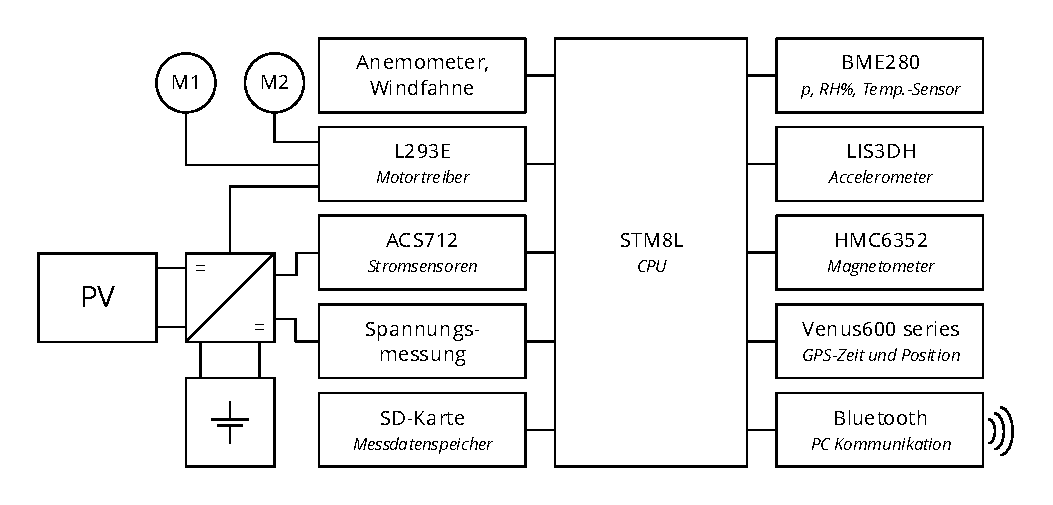
\includegraphics[width=\textwidth]{img/BSB_Uebersicht.pdf}
\end{frame}
\begin{frame}
\frametitle{Geh�use}
        
        \emph{Idee:}
        \begin{itemize}
        	\item \emph{Geh�use f�r Elektronik mittels 3D-Druck}
        	\item \emph{�berzug mit B�gelfolie}
        	\item \emph{Abdichtung der Ein- und Ausg�nge}
        \end{itemize}
        \begin{figure}
        	\flushright
        	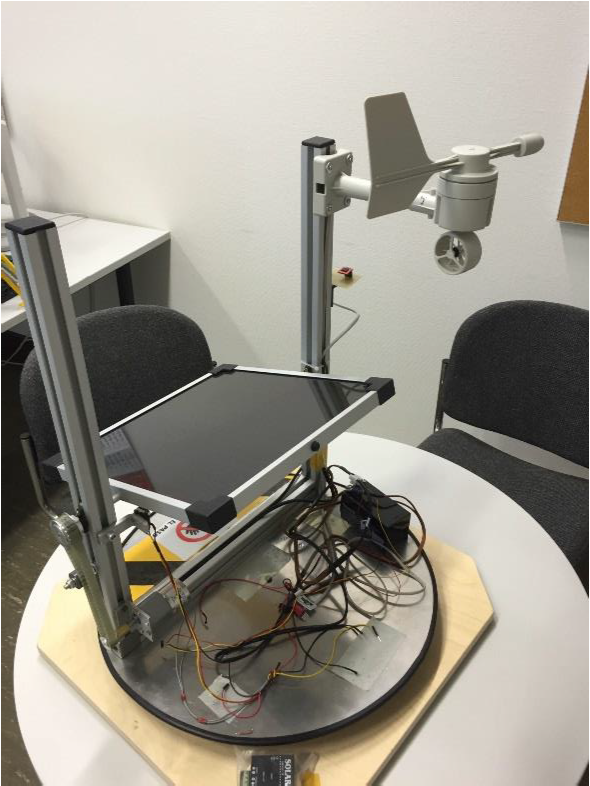
\includegraphics[width=0.3\textwidth]{img/Wetterstation_1.png}
        \end{figure}
\end{frame}

\section{Erf�llung der Anforderungen}
\begin{frame}
	\frametitle{Erf�llung der Anforderungen 1/2}
	\emph{Erf�llt}
	\begin{itemize}
		\item \emph{s�mtliche Messwerte mit Sensoren abgedeckt}
		\item \emph{zus�tzlicher Niederschlagssensor}
		\item \emph{Versorgung �ber ausgerichtetes Solarpanel}
		\item \emph{Pufferung des Ladeszustands}
		\item \emph{Positions- und H�henbestimmung mittels GPS Modul}
		\item \emph{Datenspeicherung auf microSD}
		\item \emph{Kommunikation mittels Bluetooth}
	\end{itemize}
\end{frame}

\begin{frame}
	\frametitle{Erf�llung der Anforderungen 2/2}
	\emph{Eingrenzungen}
	\begin{itemize}
		\item \emph{Arbeitsbereiche der Sensoren von -20 bis 60\ �C}
		\item \emph{Begrenzung des Standorts durch Solarpanel}
	\end{itemize}
\end{frame}

\section{Planung}
% - groben Zeitplan vorstellen (Diagramm)
\begin{frame}
  \frametitle{Aufgaben 1/2}
  \emph{Abgeschlossen:}
  \begin{itemize}
  	\item \emph{Planung der Umsetzung}
  	\item \emph{Erstellung der Aufgabenpakete}
  	\item \emph{Bestellen der Teile} %wird Montag eingereicht
  \end{itemize}
  \emph{In Arbeit:}
  \begin{itemize}
  	\item \emph{Entwurf der Spannungsversorgung}
  	\item \emph{Auswertung der Datenbl�tter}
  	\item \emph{Grundger�st der Software}
   \end{itemize} 
\end{frame}

\begin{frame}
  \frametitle{Aufgaben 2/2}
  \emph{Ausstehend:}
  \begin{itemize}
  	\item \emph{Ausrichtung des Solarpanels}
  	\item \emph{Layout Platine}
  	\item \emph{Auslesen der Sensoren}
  	\item \emph{Speichern der Messdaten}
  	\item \emph{Kommunikation mittels Bluetooth}
  	\item \emph{Anzeige auf PC (GUI)}
  	\item \emph{Montage}
  	\item \emph{Geh�use und Abdichtung}
  	\item \emph{Bericht}
  \end{itemize}  
\end{frame}

\begin{frame}[allowframebreaks]
  \frametitle{Literatur- und Quellenverzeichnis}
  \emph{Datenbl�tter der jeweiligen Sensoren}
  %\bibliographystyle{plainnat}
  %\bibliography{literature} Ich hab nicht wirklich was zitiert, sollen wir das trotzdem angeben? Daten w�ren nur aus Datenbl�ttern der Sensoren und dann die Werte f�r Druck und Temperatur, die aber Allgemeinwissen sind.
\end{frame}

\begin{frame}
\frametitle{Ende}


\begin{center}
	\Huge {\emph{Fragen?}}
\end{center}

\end{frame}

% ------------------------------------------------
% ----------------------------------------------------------------------------------------

\end{document}
%%% Local Variables:
%%% mode: latex
%%% TeX-master: t
%%% End:
